\documentclass[
	a4page,
	parskip=full,
]{scrartcl}
\usepackage[margin=2.5cm]{geometry}
\usepackage[UKenglish]{babel}
\usepackage[ddmmyyyy]{datetime}
\usepackage{libertinus, libertinust1math}
\usepackage[sfdefault]{biolinum}
\usepackage{roboto}
\usepackage{amsmath,amssymb,amsfonts,amsthm}
\usepackage{graphicx, hyperref, wrapfig, marginnote}
\usepackage[
	% sorting=none,
	% style=verbose
	style=numeric-comp, % comp = compressed 4,5,6,7 -> 4-7
	sorting=none,		% Sort by appearance
	% autocite = superscript,
	% backref=true,
	url=true
]{biblatex}
\addbibresource{literature.bib}

% decrease space after disposition
\RedeclareSectionCommands[
	afterskip=1px
]{section, subsection, subsubsection}
\renewcommand{\dateseparator}{.}

\begin{document}

{
	\sffamily\noindent
	Leon Oleschko \hfill \today\\
	Modeling Quantum Hardware: open dynamics and control \hfill Universität Konstanz\\
	\vspace*{1cm}\\
	\textbf{\Large Noise Analysis in an Optomechanical Resonance Cavity}
}

\section*{Project Proposal}
Inspired by the noise modelling techniques presented in a proposal for a gravitational wave observatory \autocite{rainer_weiss_electronically_1972},
I would like to perform a similar analysis of a noise limited experiment.
Specifically, this project will examine the standart quantum limit noise of a optomechanical resonance cavity using the numerical tools introduced in this course.

\begin{wrapfigure}{R}{3.5cm}
	\includegraphics{figures/drawing.pdf}
\end{wrapfigure}
The modelled setup consists of an optical resonator, with a harmonically moving mirror.
The mirror is thermally coupled to the environment.
The thermal coupling introduces the first type of noise, which can be modelled using the Lindblad framework presented in the lecture. 
The other sources of noise are the phase noise of the coherent states from the laser and the radiation pressure noise at the mirror. \autocite{aspelmeyer_cavity_2014-1}\\
The project can be extended by looking into modelling squeezing implementations, to minimise the measured noise \autocite{aspelmeyer_cavity_2014-1}.

The system Hamiltonian $H$ can be written as a can be written as a combination of the optical and mechanical oscillators.
The optical cavity oscillates with the frequency $\omega_\text{opt} + G \hat x$, where $\hat x$ depends on the position of the mirror position.
The mechanical oscillation is modelled harmonically with $\omega_\text{mech}$.
Therefore the Hamiltonian can be written as a harmonic and a mixing part:
\marginpar{\raggedright\small\textit{There may be some missing factors.}}
\marginpar{\raggedright\small\textit{Or even a missing term.}}
$$
	H = \underbrace{
		a^\dagger a\; (\omega_\text{opt} + G \hat x)
	}_{\text{optical}}+ \underbrace{
		b^\dagger b\; \omega_\text{mech}
	}_{\text{mechanical}}
	= 
	\underbrace{
			a^\dagger a\; \omega_\text{opt}
		+ b^\dagger b\; \omega_\text{mech}
	}_{\text{harmonic}}
	+ 
	\underbrace{
		G\; a^\dagger a\; (b^\dagger + b)
	}_{\text{coupling}}
$$ 

Then using the Lindblad jump operators thermal noise, a driving laser and the measurement can be modelled.
The thermal noise can be modelled in the same way it was done in the lecture.
The driving laser has the effect of adding a coherent state in every time interval.
The phase can be measured in a way that introduces radiation pressure into the mechanical oscillator, this is discussed in \autocite{aspelmeyer_cavity_2014}.

Modelling a quantum system using a Hamiltonian and Lindblad jump operators is a common technique, that was also discussed in the lecture.
Many numerical implementations for this framework exist.

The goal of the project is to demonstrate the standart quantum limit in the described setup.
This is a combination of Shot Noise, radiation pressure and thermal noise.

As an extension it can be demonstrate that choosing a better driving field allows to squeeze the measurement noise bellow the quantum limit.


\printbibliography


\end{document}
